\chapter{Modelling DISFA} \label{sec:model}
  This chapter describes the path taken in constructing the autoencoding classifier (AEC) network, detailing
  the experiments which were performed to create the final configuration.
  The most important metric used to judge a network in the chapter is this Average ROC score of the classifier
  when applied to the un-seen test set, the secondary metric is the error
  in the reconstructed image outputted from the autoencoder. The overall aim is to
  find a configuration where the presence of the autoencoder improves
  the performance of the classifier and secondarily where improving the secondary metric (the autoencoder) improves
  the primary metric (the classifier).

  \begin{figure}[h!]
   \centering
   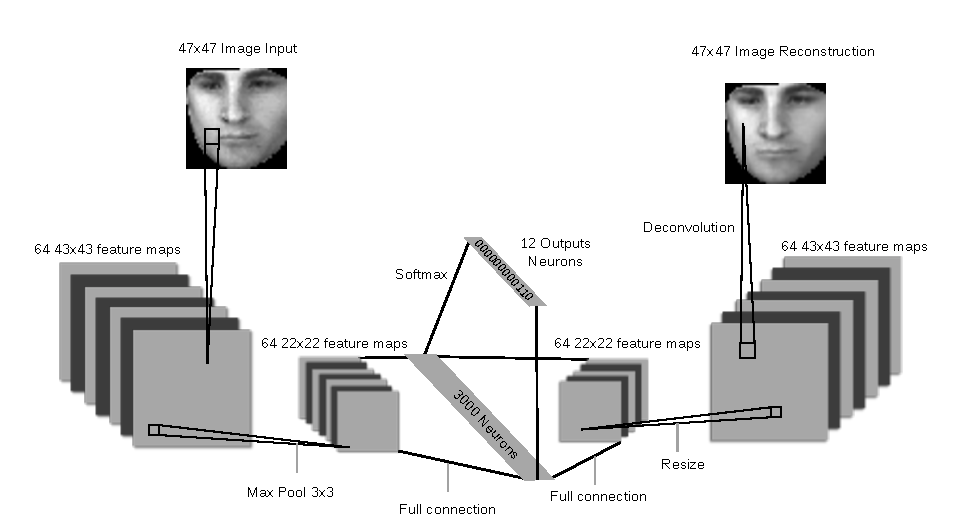
\includegraphics[width=\textwidth]{illustrations/aec_network.pdf}
   \captionof{figure}{A diagram of network 2 used in this section.}
  \end{figure}

  The results will show, that it is unclear if there is a direct relationship between optimising the two objective functions, nonetheless
  the work is a detailed exploration of how autoencoders and classifiers can interact with each other
  under various preprocessing situations and different autoencoder transfer functions \footnote{These describe the degree to which
  each cost function is trained during training, see section \ref{sec:autoalpha}.}.

  \section{Experimental set up}
    In order to develop the network for modelling the DISFA dataset a set of common
    parameters for experimentation are useful to define, these are shown in table \ref{tab:common}

    \begin{table}[!h]
      \centering { \footnotesize
      \begin{tabular}{ll}
        \hline
        \textbf{Parameter}                       & \textbf{Value}                \\ \hline
        Optimizer                                & Adam                          \\
        Learning Rate                            & 0.001                         \\
        L2 Regularisation Coefficient            & 0.0                           \\
        Hidden layer activation functions         & Leaky ReLu                          \\
        Image downscaling                        & 0.4                           \\
        AU's present                             & 1,2,4,5,6,9,12,15,17,20,25,26 \\
        Iterations:                              & 1000                          \\
        Early model save percent                 & 50\%                          \\
        Weight tensor initial standard deviation & 0.001                         \\
        Bias tensor initial value                & 0.01                          \\
        Train batch size                         & 100                           \\
        Validation batch size                    & 500                           \\
        Penultimate fully connected layer size   & 3000                          \\
        Autoencoder cost function                & Mean Squared Error            \\
        Classifier cost function                 & Cross Entropy                 \\
        \hline
      \end{tabular}
      \caption{Common parameters for most experiments in the section. These parameters should be
      assumed in proceeding sections unless otherwise stated.} \label{tab:common} }
    \end{table}

    The cost functions were chosen as they are typical of their use cases, the cross entropy is more suited
    for classification problems as it penalises heavily incorrect answers and the meaned squared

    For all of the experiments the data was partitioned in a 50/50 split as shown in table \ref{sec:splitting}:
    \begin{table}[h!]
      \centering { \footnotesize
      \begin{tabular}{|l|l|}
      \hline
      Set & Subjects   \\
      \hline
       Train          & 2,4,6,8,10,12,16,18,23,25,27,29,31      \\
      \hline
      Validation      & 1,3,5,7,9,11,13,17,21,24,26,28,30,32 minus test set     \\
      \hline
      Test           & 500 chosen randomly taken from validation set      \\
     \hline
      \end{tabular}
      \caption{The split of the DISFA dataset used in the experiments.}
      \label{sec:splitting} }
    \end{table}

    For the labels AU intensities 1-5 counted as a postive example and AU intesnity 0 counted as a negative one.
    No examples were removed from the training set.

  % A single hidden layer
  % A single hidden layer
  % A single hidden layer
  % A single hidden layer
  \section{A single hidden layer}
    \begin{table}[h!]
    \centering
    {\footnotesize
    \begin{tabular}{|lllllllll|}
    \hline
    \multicolumn{1}{|l|}{Element} & Type     & \multicolumn{1}{l|}{Dimensions}                     & Type     & \multicolumn{1}{l|}{Dimensions}                      \\ \hline
    \multicolumn{1}{|l|}{x}       &          & \multicolumn{1}{l|}{$47\times47\times1$}            &          & \multicolumn{1}{l|}{}                                \\ \hline
    \multicolumn{1}{|l|}{$L_1$}   & fc       & \multicolumn{1}{l|}{$2209\times14$}              & Binary Softmax & \multicolumn{1}{l|}{$3000\times2\times12$}        \\
    \multicolumn{1}{|l|}{$y_1$}   & dropout  & \multicolumn{1}{l|}{$14$}                         &          & \multicolumn{1}{l|}{$24$}                              \\ \hline
    \multicolumn{1}{|l|}{$L_2$}   & fc       & \multicolumn{1}{l|}{$14\times2209$}              &          & \multicolumn{1}{l|}{}                                   \\
    \multicolumn{1}{|l|}{$y_2$}   &          & \multicolumn{1}{l|}{$3000$}                         &          & \multicolumn{1}{l|}{}                                \\ \hline
    \multicolumn{1}{|l|}{$L_3$}   & reshape & \multicolumn{1}{l|}{}                    &          & \multicolumn{1}{l|}{}                                \\
    \multicolumn{1}{|l|}{$y_3$}   &          & \multicolumn{1}{l|}{$47\times47\times 1$}          &          & \multicolumn{1}{l|}{}                                \\ \hline
    \end{tabular}

    \caption{} \label{net:simple1}

    }
    \end{table}
    %ID = 4 date = '2016_08_14' group = 'alpha'
    As an introduction to the types of results that will be used to evaluate various
    models, this section shows the performance of a neural network with one
    hidden layer. This also should provide a worst case for classification and autoencoding performance.

    The structure of this network is shown in table \ref{net:simple1}, 14 neurons
    are chosen heuristically as there are 14 AU's and one might naively hope that the number of
    neurons required in the hidden layer would be equal to the number of features. Per subject face normalisation
    is chosen from section \ref{sec:meanface} and the images are scaled to be size $118 \times 118$.
    Figure \ref{fig:simple} shows the losses during training, on the train and validation set where table \ref{tab:splitting}
    describes the way the data is partitioned. Over fitting to the train set is evident very early in the training, there are two
    possible reasons, firstly the validation set might be too small to represent all AUs that are being learnt and secondly the train
    set contains different subjects so this will cause a potentially unavoidable amount of overfitting.
    Training the classifier reduces the performance of the autoencoder on the
    training set visibly but interestingly not for the validation set.

    \begin{table}[h!]
      \centering
      {\footnotesize
      \begin{tabular}{|l|l|}
      \hline
      set & subjects   \\
      \hline
       Train          & 2,4,6,8,10,12,16,18,23,25,27,29,31      \\
      \hline
      Test      & 1,3,5,7,9,11,13,17,21,24,26,28,30,32 minus validation set     \\
      \hline
      Validation           & 500 chosen randomly taken from test set      \\
     \hline
      \end{tabular}
      \caption{Typical split of the DISFA dataset for experimentation purposes}
      \label{tab:splitting}  }
    \end{table}


    \begin{figure}[!h]
    \centering
    \includegraphics[width =\hsize]{../graphs/losses_2016_08_14_004.pdf}
    \caption{The losses of a neural network consisting of a $118^2$ neuron input layer, a 14
    neuron hidden layer, a branch of the same size as the input layer for autoencoding
    and branches for binary softmax classifiers for each AU. The network trains by minimising
    the cross entropy. The $\alpha$ coefficient determines the balance between the
    classifier and the autoencoder losses, $\alpha=1$ signifies only autoencoder training
    while $\alpha=0$ means only classifier training. Over fitting is observed
    on all loss functions. Training the classifier
    overwrites the weights and hence ends up reducing
    the performance of the autoencoder however the
    model is so simple that the validation set remains almost constant.}
    \label{fig:simple}
    \end{figure}

    \begin{table}[!h]
    \centering
    {\small
    \begin{tabular}{llllll}
    \hline
    \textbf{Class}    & \textbf{ROC} & \textbf{ROC Ranking} & \textbf{Max F1} & \textbf{Max Precision} & \textbf{Max Recall} \\ \hline
    1                 & 0.50         & fail         & 0.09            & 0.06                   & 1.0                 \\
    2                 & 0.60         & poor         & 0.07            & 0.05                   & 1.0                 \\
    4                 & 0.62         & poor         & 0.31            & 0.27                   & 1.0                 \\
    5                 & 0.49         & fail         & 0.02            & 0.02                   & 1.0                 \\
    6                 & 0.80         & fair         & 0.48            & 0.42                   & 1.0                 \\
    9                 & 0.46         & fail         & 0.11            & 0.06                   & 1.0                 \\
    12                & 0.89         & good         & 0.67            & 0.73                   & 1.0                 \\
    15                & 0.46         & fail         & 0.11            & 0.06                   & 1.0                 \\
    17                & 0.55         & fail         & 0.18            & 0.25                   & 1.0                 \\
    20                & 0.51         & fail         & 0.09            & 0.12                   & 1.0                 \\
    25                & 0.65         & poor         & 0.51            & 0.42                   & 1.0                 \\
    26                & 0.57         & fail         & 0.32            & 0.23                   & 1.0                 \\ \hline
    \textbf{Average:} & 0.59         & fail         & 0.25            & 0.22                   & 1.0                 \\ \hline
    \end{tabular} }
    \caption{The final evaluation for the training session shown in \ref{fig:simple}.
    AU 12 and 6 are the only AUs learnt well. These values were
    calculated on the test set. The maximum F1, Precision and Recalls
    were found by trying 20 threshold values between 0 and 1.}
    \label{my-label}
    \end{table}


    \newpage
    %
    %
    %
    %
  \section{Joint classification}

    Typical deep neural networks are used to classify
    one image into only one category. The case with FAU detection is different, we
    would like to be able to classify the categories jointly,  putting one frame into more than
    one AU category. Ideally the network would output a confidence score between 0 and 1
    to signify if an AU is present and we would calculate some optimum threshold value
    (ideally this would be 0.5).

    The following list details three possible solutions to the joint classification problem:

    \begin{itemize} \label{sec:binsoft}
      \item {\bf Softmax Layer} - This is a traditional, fully connected layer with
                                  a softmax activation function (see equation \ref{eq:softmax}).
                                  The issue with this is that it provides a probability distribution over AUs
                                  but the required quantity is a probability distribution for each AU.
      \item {\bf Sigmoid Layer} - This again is like the previous solution but instead each neuron gives a confidence
                                  score between 0 and 1 for each AU with a sigmoid function (see equation \ref{eq:sigmoid}).
                                  The issue with this however is that sigmoid
                                  functions have vanishing gradients at large input values
                                  hence training may become difficult.
      \item {\bf Binary Softmax Layers} - Here there is a two neuron softmax layer
                                          for each AU, this doubles the amount of weights
                                          but gives a probability over the presence and
                                          absence of each AU which is ideal. In the implementation
                                          the negative neuron of each binary layer is only used for training purposes, and it is
                                          discarded while evaluating the classification performance.
    \end{itemize}

    Table \ref{net:classcompnet} compares how each of these solutions perform using the network described in
    tables \ref{tab:binsoftcomp}, this network was chosen because it contains all of the main
    components of larger networks typically used for classification tasks, such as a convolutional
    layer, max pool layer and fully connected layer. It contains the autoencoder section which will be
    explored later on in the section mainly out of interest.

    \begin{table}[h!]
    \centering
    {\footnotesize
    \begin{tabular}{|lllllllll|}
    \hline
    \multicolumn{1}{|l|}{Element} & Type     & \multicolumn{1}{l|}{Dimensions}                     & Type     & \multicolumn{1}{l|}{Dimensions} \\ \hline
    \multicolumn{1}{|l|}{x}       &          & \multicolumn{1}{l|}{$47\times47\times1$}            &          & \multicolumn{1}{l|}{}          \\ \hline
    \multicolumn{1}{|l|}{$L_1$}   & conv 1   & \multicolumn{1}{l|}{$5\times 5\times1\times 64$}    &          & \multicolumn{1}{l|}{}          \\
    \multicolumn{1}{|l|}{$y_1$}   &          & \multicolumn{1}{l|}{$43\times43\times64$}           &          & \multicolumn{1}{l|}{}          \\ \hline
    \multicolumn{1}{|l|}{$L_2$}   & max pool & \multicolumn{1}{l|}{$2\times 2$}                    &          & \multicolumn{1}{l|}{}          \\
    \multicolumn{1}{|l|}{$y_2$}   &          & \multicolumn{1}{l|}{$22\times22\times 64$}          &          & \multicolumn{1}{l|}{}          \\ \hline
    \multicolumn{1}{|l|}{$L_3$}   & fc       & \multicolumn{1}{l|}{$30976\times3000$}              & \multicolumn{2}{l|}{Sotmax Layer or}      \\
    \multicolumn{1}{|l|}{$y_3$}   &          & \multicolumn{1}{l|}{}                               & \multicolumn{2}{l|}{Sigmoid Layer or}     \\
    \multicolumn{1}{|l|}{$L_4$}   & dropout  & \multicolumn{1}{l|}{$3000$}                         & \multicolumn{2}{l|}{Binary Softmax Layer} \\
    \multicolumn{1}{|l|}{$y_4$}   &          & \multicolumn{1}{l|}{}                               &          & \multicolumn{1}{l|}{}          \\ \hline
    \multicolumn{1}{|l|}{$L_5$}   & resize\& reshape & \multicolumn{1}{l|}{$2$}                    &          & \multicolumn{1}{l|}{}          \\
    \multicolumn{1}{|l|}{$y_5$}   &          & \multicolumn{1}{l|}{$43\times43\times 64$}          &          & \multicolumn{1}{l|}{}          \\ \hline
    \multicolumn{1}{|l|}{$L_6$}   & deconv 1   & \multicolumn{1}{l|}{$5\times 5\times1\times 64$}  &          & \multicolumn{1}{l|}{}\\
    \multicolumn{1}{|l|}{$y_6$}   &          & \multicolumn{1}{l|}{$47\times47\times1$}            &          & \multicolumn{1}{l|}{}         \\ \hline
    \end{tabular}

    \caption{Set up for deciding on which final layer structure to use.
    This network is very similar to \textbf{Network 1} which is described later in the section.} \label{net:classcompnet}

    }
    \end{table}


    \begin{table}[!h] {\footnotesize
      \centering
      \begin{tabular}{lccc}
      \hline
      Final Layer   & Av. ROC &   Av. Best F1 &   Autoencoder Loss (Not normalised) \\
      \hline
      Binary Softmax Layers  &   0.73 &  0.34 &   20.7 \\
      Softmax Layer          &   0.69 &  0.30 &   15.8 \\
      Sigmoid Layer          &   0.50 &  0.19 &  126.2 \\
      \hline
      \end{tabular}
    \caption{Comparison of the three ways the final layer could be implemented using network 2 (see table \ref{net:classcompnet}). The
    preprocessing method used was face normalisation (not per subject). 500 iterations were used. } \label{tab:binsoftcomp} }
    \end{table}

    The results show that the binary softmax layer outperforms the other solutions. The
    softmax layer is only slightly worse, but in order to accommodate for the potential of higher rates
    it is clear that the binary softmax is the better choice. This is because, in joint classification problems
    the simple softmax layer struggles to report more than 2 AU's as the outputs must add up to one.
    The low performance of the sigmoid layer is interesting and one reason might be that of vanishing gradients due to
    the bottleneck layer containing high activation values.

    As the softmax layer is better in the results and has a better potential for good results
    it is chosen as the classifier for the following experiments.

  %
  %
  %
  %
  \section{Autoencoder classifier balancing} \label{sec:autoalpha}
    A key structure that is to be investigated in this report is a network with two objective functions:
    autoencoder and classifier. This is achieved by having a bottleneck layer where the branching occurs.
    The autoencoder has symmetry along this bottleneck, while the classifier consists of one further layer
    (the binary softmax classifier from the previous section). The cost function for the whole network is as follows:

    \begin{equation}
        J(\tilde{\mathbf{x}},\tilde{\mathbf{y}}) = -\frac{1-\alpha(t)}{2FN_B}\tilde{\mathbf{y}}\cdot\log(\mathbf{y}(\tilde{\mathbf{x}}))
        + \frac{\alpha(t)}{N_BN_P}\left |\mathbf{y}(\tilde{\mathbf{x}}) \odot \mathbf{M}-\tilde{\mathbf{x}}\right | ^2
    \end{equation}

    Where $\mathbf{M}$ is a mask described in section \ref{sec:mask}. Here F is the number of AU's, N is the size of the batch and $\alpha(t)$ is a
    function which balances the two costs. $\alpha(t)$ might be constant $\left ( \alpha_{\text{constant}}(t)=\frac{1}{2} \right )$ or
    some sort of polynomial which stays in the range $[0,1]$. $N_B$ and $N_P$ are the batch size and number of pixels respectively.

    For much of the initial investigations we employ:
    \begin{equation}
    \alpha_{\text{step}}(t,p,T) =
    \begin{cases}
      1           & \text{if}\ t<pT \\
      0           & \text{otherwise}
    \end{cases}
    \end{equation}

    Where $t$ indexes iterations, $T$ is the total number of iterations and p is the
    percentage of iterations that should be in the first region of the piecewise function
    where $\alpha=1$.
    This nicely expresses what is typically meant by pre-training in the literature, it trains
    the autoencoder up until iteration $pT$ (normally $p=\frac{1}{2}$ or $p=\frac{2}{3}$) and then the classifier for the remainder of the time.
    This acts as a good base case to test both sides of the network, later more interesting
    functions will be explored such as the sigmoid step:

    \begin{equation}
      \alpha_{\text{sigmoid}}(t,T,p,\tau) = \frac{1}{1 + \exp(1 + \tau (t/T - p))}
    \end{equation}

    Or a polynomial function:

    \begin{equation}
      \alpha_{\text{poly}}(t,T,n) = 1 - \left ( \frac{t}{T} \right )^n
    \end{equation}

    Or a periodic step function:

    \begin{equation}
    \alpha_{\text{alternate}}(t,T,p) =
    \begin{cases}
      1           & \text{if } t < |T/p| \text{ and } p > 0\\
      0           & \text{if } t < |T/p| \text{ and } p \leq 0\\
      \alpha_{\text{alternate}}(t-|T/p|,T,-p)           & \text{otherwise} \\
    \end{cases}
    \end{equation}

    Examples of such functions are plotted in figure \ref{fig:alpha_functions}.

    \begin{figure}[!h]
    \centering
    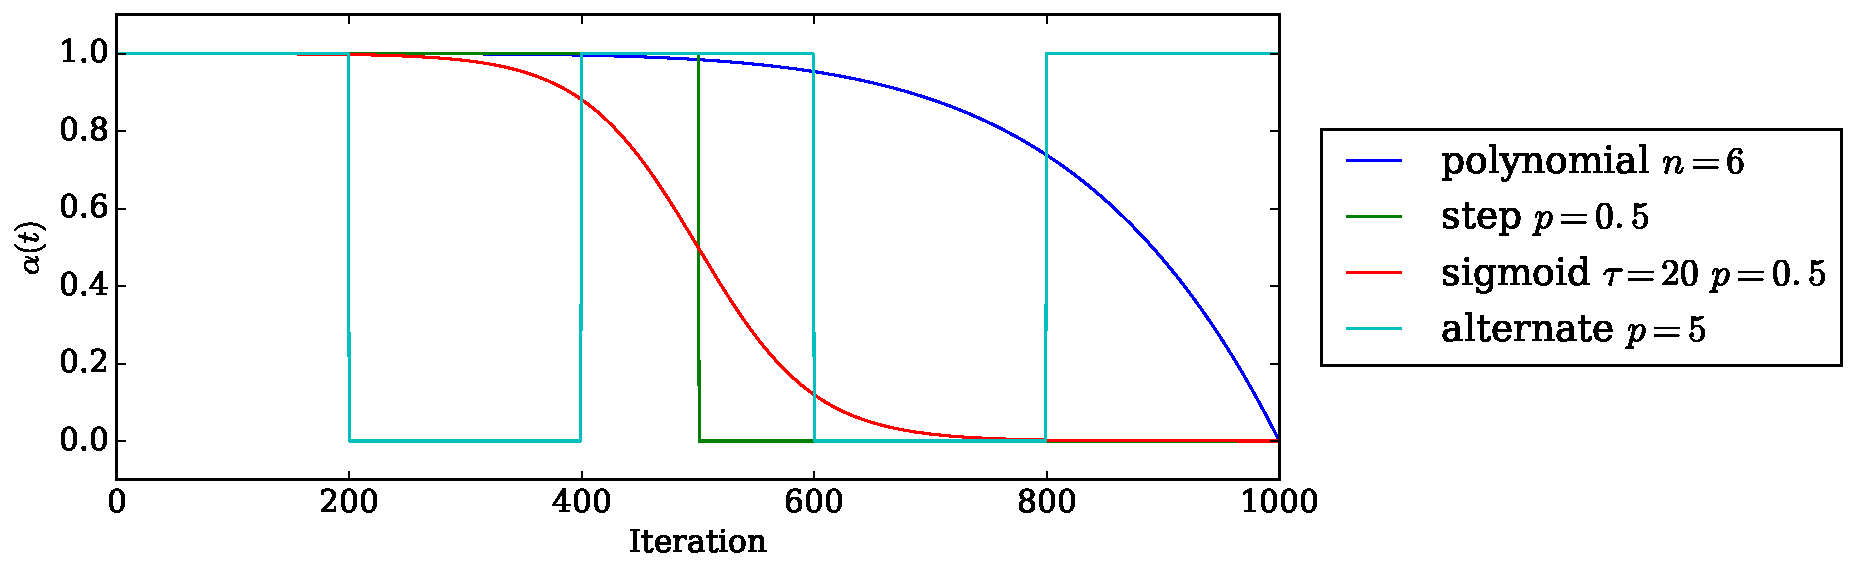
\includegraphics[width =\hsize]{figures/alpha.pdf}
    \caption{Examples of alpha transfer functions described in section \ref{sec:autoalpha}.
    For the polynomial case higher values of $n$ decrease the amount of training
    the classifier receives. While in the case of the step p dictates the training
    that each network receives, the sigmoid can be seen as a smoothed out step function
    with the two being equivalent as $ \tau \rightarrow \infty$. Similarly as $n \rightarrow \infty$
    the polynomial function turns into a constant function with $c=1$ except at the final
    iteration.}
    \label{fig:alpha_functions}
    \end{figure}

    % def alpha_sigmoid(_x,_N,a=20,b=0.5):
    %     x = float(_x)
    %     N = float(_N)
    %     arg = x/N - b
    %     return 1.0/(1.0 + exp(a*arg))

  %
  %
  %
  %
  %
  \newpage
  \section{Convolutional Networks}

    Now that some basic structures have been tested we proceed to convolutional networks,
    inspired by the literature (see table \ref{tab:compnet}) three networks are defined.
    Network 2 is shown in table \ref{tab:net2}, Network 3
    adds another convolutional layer of size $5\times 5 \times 64 \times 64$ to this and
    Network 4 adds a $4\times 4 \times 64 \times 128$ layer
    on top of Network 3. Regarding the decoder section the inverse operations are
    performed, see appendix \label{appendix1} for full details
    for networks 2,3 and 4.

    % network.append(cnn_layer(ll(network), [5, 5, 64, 64], 'VALID', 'Convolution_2', config, act=act))
    % network.append(cnn_layer(ll(network), [4, 4, 64, 128], 'VALID', 'Convolution_3', config, act=act))

    \begin{table}[h!] \caption*{\textbf{Network 2}}
    \centering
    {\footnotesize
    \begin{tabular}{|lllllllll|}
    \hline
    \multicolumn{1}{|l|}{Element} & Type     & \multicolumn{1}{l|}{Dimensions}                     & Type     & \multicolumn{1}{l|}{Dimensions}  \\ \hline
    \multicolumn{1}{|l|}{x}       &          & \multicolumn{1}{l|}{$47\times47\times1$}            &          & \multicolumn{1}{l|}{}            \\ \hline
    \multicolumn{1}{|l|}{$L_1$}   & conv 1   & \multicolumn{1}{l|}{$5\times 5\times1\times 64$}    &          & \multicolumn{1}{l|}{}            \\
    \multicolumn{1}{|l|}{$y_1$}   &          & \multicolumn{1}{l|}{$43\times43\times64$}           &          & \multicolumn{1}{l|}{}            \\ \hline
    \multicolumn{1}{|l|}{$L_2$}   & max pool & \multicolumn{1}{l|}{$2\times 2$}                    &          & \multicolumn{1}{l|}{}            \\
    \multicolumn{1}{|l|}{$y_2$}   &          & \multicolumn{1}{l|}{$22\times22\times 64$}          &          & \multicolumn{1}{l|}{}            \\ \hline
    \multicolumn{1}{|l|}{$L_3$*}   & fc       & \multicolumn{1}{l|}{$30976\times3000$}              & Binary
                                                                                                      Softmax & \multicolumn{1}{l|}{$3000\times2\times12$}        \\
    \multicolumn{1}{|l|}{$y_3$}   & dropout  & \multicolumn{1}{l|}{$3000$}                         &          & \multicolumn{1}{l|}{$24$}        \\ \hline
    \multicolumn{1}{|l|}{$L_4$}   & fc       & \multicolumn{1}{l|}{$3000\times30976$}              &          & \multicolumn{1}{l|}{}            \\
    \multicolumn{1}{|l|}{$y_4$}   &          & \multicolumn{1}{l|}{$3000$}                         &          & \multicolumn{1}{l|}{}            \\ \hline
    \multicolumn{1}{|l|}{$L_5$}   & resize\& reshape & \multicolumn{1}{l|}{$2$}                    &          & \multicolumn{1}{l|}{}            \\
    \multicolumn{1}{|l|}{$y_5$}   &            & \multicolumn{1}{l|}{$43\times43\times 64$}          &          & \multicolumn{1}{l|}{}            \\ \hline
    \multicolumn{1}{|l|}{$L_6$}   & deconv 1   & \multicolumn{1}{l|}{$5\times 5\times1\times 64$}  &          & \multicolumn{1}{l|}{}            \\
    \multicolumn{1}{|l|}{$y_6$}   &            & \multicolumn{1}{l|}{$47\times47\times1$}            &          & \multicolumn{1}{l|}{}             \\ \hline
    \end{tabular}

    \caption{A network used many times in the report, for further details see appendix \ref{appendix1} \label{tab:net2}
    \newline *Bottleneck layer}
    }
    \end{table}

    %
    %
    %
    %
    %
    \newpage
    \section{Preprocessing methods} \label{sec:psearch}

      With the goal of creating the AEC network a search on some hyperparameters was performed
      including the preprocessing method from section \ref{sec:methods} and on the four main activation functions
      that are typically used on the last layer of an autoencoder (linear, ReLU, sigmoid and tanh), table \ref{tab:psearch} shows the results.
      These parameters cover a lot of possible configurations and should have markedly different results, the idea
      is that the encoding at the bottleneck layer should be different for each set of parameters and that
      one of these might offer a good starting set of weights for the classifier to train from.

      \begin{table}[!h] {\footnotesize
        \centering
      \begin{tabular}{lllrrrrrr}
            && &   \multicolumn{3}{|c|}{Autoencoder Training} &  \multicolumn{3}{c|}{Classifier Training}    \\
        \hline
         i&Preprocessing    & Activation Function&  ROC&F1&AE Loss & ROC & F1 & AE Loss \\
         \hline
         1&Per Subject Contrast Face & linear &    0.49 &   0.19 &     0.12 &    0.82 &   0.46 &     0.18 \\
         2&Per Subject Contrast Face & tanh   &    0.49 &   0.19 &     0.12 &    0.82 &   0.46 &     0.13 \\
         3&Per Subject Contrast Face & relu   &    0.63 &   0.19 &     0.12 &    0.81 &   0.44 &     0.14 \\
         4& Per Subject Contrast Face & sigmoid &    0.52 &   0.2  &     0.13 &    0.08 &   0.19 &     0.13 \\
         \hline
         5&Contrast          & linear &    0.40 &   0.19 &     0.19 &    0.74 &   0.34 &     1.46 \\
         6&Contrast          & tanh   &    0.61 &   0.19 &     0.20 &    0.72 &   0.35 &     0.35 \\
         7&Contrast          & relu   &    0.59 &   0.19 &     0.25 &    0.75 &   0.36 &     0.65 \\
         8& Contrast         & sigmoid &    0.54 &   0.19 &     0.22 &    0    &   0.19 &     0.28 \\
         \hline
         9&Face              & linear &    0.46 &   0.19 &     0.06 &    0.73 &   0.35 &     0.26 \\
         10&Face              & tanh   &    0.52 &   0.19 &     0.08 &    0.74 &   0.35 &     0.13 \\
         11&Face              & relu   &    0.45 &   0.19 &     0.09 &    0.73 &   0.36 &     0.35 \\
         12& Face             & sigmoid &    0.47 &   0.2  &     0.1  &    0.72 &   0.35 &     0.13 \\
         \hline
         \hdashline
         13&Per Subject Face  & linear &    $0.64$ &   $0.19$ &     $0.03$ &    $0.83$ &   $0.48$ &     $0.12$ \\
         &{\it error:}  &&$\pm$0.02 &$\pm$0.01 &$\pm$0.02  &$\pm$0.02 &$\pm$0.01 &$\pm$0.02 \\
         \hdashline
         14&Per Subject Face  & tanh   &    0.56 &   0.19 &     0.03 &    0.81 &   0.47 &     0.05 \\
         15&Per Subject Face  & relu   &    0.56 &   0.19 &     0.04 &    0.81 &   0.48 &     0.11 \\
         16& Per Subject Face      & sigmoid &    0.62 &   0.23 &     0.04 &    0.81 &   0.46 &     0.05 \\
         \hline
         17&Range [-1,1]      & linear &    0.50 &   0.19 &     0.07 &    0.73 &   0.35 &     3.90 \\
         18&Range [-1,1]      & tanh   &    0.54 &   0.19 &     0.07 &    0.75 &   0.35 &     0.30 \\
         19&Range [-1,1]      & relu   &    0.48 &   0.19 &     0.15 &    0.73 &   0.35 &     4.73 \\
         20& Range [-1,1]      & sigmoid &    0.49 &   0.2  &     0.12 &    0.73 &   0.31 &     0.36 \\
         \hline
         21&None              & linear &    0.51 &   0.19 &     0.08 &    0.74 &   0.34 &     4.02 \\
         22&None              & tanh   &    0.59 &   0.19 &     0.07 &    0.71 &   0.33 &     0.93 \\
         23&None              & relu   &    0.53 &   0.19 &     0.20 &    0.53 &   0.23 &     0.41 \\
         24& None       & sigmoid &    0.47 &   0.19 &     0.09 &    0.65 &   0.29 &     0.46 \\
         \hline
         25&Contrast Face     & linear &    0.56 &   0.19 &     0.24 &    0.74 &   0.35 &     0.40 \\
         26&Contrast Face     & tanh   &    0.54 &   0.19 &     0.24 &    0.75 &   0.38 &     0.26 \\
         27&Contrast Face     & relu   &    0.54 &   0.19 &     0.25 &    0.74 &   0.35 &     0.35 \\
         28& Contrast Face    & sigmoid &    0.44 &   0.19 &     0.25 &    0.71 &   0.34 &     0.26 \\
         \hline
        \end{tabular}
          \caption{Comparison of four activation functions for the autoencoder for each type of preprocessing method.
          No significant difference is seen between the activation functions apart from with the sigmoid
          which makes training the classifier fail completely.
          Error values are required because tensorflow does implement fully deterministic
          processing with GPU cards (see section \ref{sec:GPU} the values in the errors were
          calculated by rerunning experiment 13 5 times. The autoencoder losses were calculated
          by first applying the inverse transform of the preprocessing method and then taking the mean squared
          difference between the reconstructed image and original image. {\bf Experimental Configuration:}
          The alpha function is $\alpha(t)=\alpha_{\text{step}}(t,0.5,1000)$.
          meaning the autoencoder training runs for 500 iterations and then the classifier for 500.
          The network is described in table \ref{tab:net2} and the training datasets are split in half as in section
          \ref{sec:splitting}.}
      \label{tab:psearch} }
      \end{table}

      The highest ROC and F1 score is found in experiment 13 in table \ref{tab:psearch}. Experiment 12
      has effectively the same score and a lower final autoencoder loss, but it uses the tanh activation
      function and hence cannot fully reconstruct the input image which has values well outside the
      range $[-1,1]$ hence linear activation function is chosen to ensure the potential for full reconstruction is there.
      Also since this preprocessing method encodes high activations as AUs these should be
      an importnt focus of the reconstruction, the tanh functions might focus more on the smaller values which
      do not encode as much AU information.

    %
    %
    %
    %
    %
    \newpage
    \section{Shared Weights}
      In order to reduce the number of parameters in an autoencoder, to avoid over fitting
      and the probability of learning the identity function, it is often helpful to share weights
      between the encoder and decoder sections.
      Table \ref{tab:sharedweights} shows
      for three networks the effect of having and not having shared weights.

      \begin{table}[!h] \centering
      {\footnotesize
      \begin{tabular}{rrllrrrrrrrr}
        &&&&   \multicolumn{3}{|c|}{Autoencoder Training} &  \multicolumn{3}{c|}{Classifier Training}    \\
      \hline
        i & Network               &   Shared Weights &    ROC&F1&AE Loss & ROC & F1 & AE Loss \\
      \hline
       1 & 2    & False     &    0.38 &   0.19 &     0.03 &    0.79 &   0.45 &     0.05 \\
       2 & 2    & True      &    0.48 &   0.19 &     0.02 &    0.81 &   0.48 &     0.12 \\
      \hline
      4 & 3    & False     &    0.55 &   0.19 &     0.03 &    0.78 &   0.41 &     0.06 \\
      5 & 3    & True      &    0.56 &   0.19 &     0.02 &    0.8  &   0.46 &     0.18 \\
      \hline
      8 & 4     & False     &    0.54 &   0.19 &     0.03 &    0.77 &   0.38 &     0.05 \\
      9 & 4     & True      &    0.42 &   0.19 &     0.03 &    0.78 &   0.42 &     1.37 \\
       \hline
     \end{tabular}}\caption{A simple experiment showing that using shared weights is beneficial
     to both autoencoder loss and classification performance. {\bf Experimental Configuration:}
      The alpha function is $\alpha(t)=\alpha_{\text{step}}(t,0.5,1000)$.
      meaning the autoencoder training runs for 500 iterations and then the classifier for 500.
      The network is described in table \ref{net:classcompnet} and the training datasets are split in half as in section
      \ref{sec:splitting}.} \label{tab:sharedweights} \end{table}

      It can be seen that using shared weights consistently improves the classification
      performance by a small amount and in some cases the autoencoder performance. After the classifier has
      damaged the autoencoder, as expected, the shared weight cases suffers a much higher loss. This is
      because the classifier does not have access to the decoder weights if the weights are not shared and hence
      changes fewer of the autoencoders parameters. The following sections all use shared weights due to this result.
    %
    %
    %
    %
    %
    \newpage
    \section{Local Contrast Normalisation}

      The local contrast normalisation scheme as described in section \ref{sec:lrn}
      was applied to the three test networks.

      \begin{table}[!h] \centering
        \footnotesize{
        \begin{tabular}{rrllrrrrrrrr}
          &&&   \multicolumn{3}{|c|}{Autoencoder Training} &  \multicolumn{3}{c|}{Classifier Training}    \\
        \hline
          i & Network             & LRN Layers   &    ROC&F1&AE Loss & ROC & F1 & AE Loss \\
        \hline
         1 & 2 & 0  &    0.48 &   0.19 &     0.02 &    0.81 &   0.48 &     0.12 \\
         2 & 2 & 1  &    0.49 &   0.19 &     0.02 &    0.81 &   0.47 &     0.13 \\
        \hline
         3 & 3 & 0  &    0.56 &   0.19 &     0.02 &    0.8  &   0.46 &     0.18 \\
         4 & 3 & 1  &    0.57 &   0.19 &     0.02 &    0.8  &   0.46 &     0.19 \\
         5 & 3 & 2  &    0.52 &   0.19 &     0.02 &    0.8  &   0.45 &     0.22 \\
        \hline
         6 & 4 & 0  &    0.42 &   0.19 &     0.03 &    0.78 &   0.42 &     1.37 \\
         7 & 4 & 1  &    0.52 &   0.19 &     0.03 &    0.79 &   0.44 &     1.02 \\
         8 & 4 & 2  &    0.52 &   0.19 &     0.03 &    0.8  &   0.44 &     0.88 \\
        \hline
        \end{tabular}}

        \caption{Results for applying local contrast normalisation layers
        for the three test networks. LRN Layers 0 means no LRN, 1 means a LRN layer is added after the max pool
        and 2 means a LRN layer is added at the final convolutional layer in the encoder. There is no
        inverse for LRN and hence the decoder section remains unchanged. {\bf Experimental Configuration:} see caption
        for table \ref{tab:sharedweights}
        }
        \label{tab:lrn}
      \end{table}

      Table \ref{tab:lrn} provides some improvement in performance for network 4 and seems
      not to effect the other networks by much. It is interested that the larger network
      is less likely to reduce autoencoder loss with the LRN layers.

      \newpage
    %
    %
    %
    %
    %
    %
    \newpage
    \section{Dropout}
      Varying degrees of dropout (see section \ref{sec:dropout}) were applied to each test network at the bottleneck layer.
      Table \ref{tab:dropout} shows the results.
      \begin{table}[h]
      \centering
      { \footnotesize
      \begin{tabular}{rllrrrrrrrr}
                           &         &                                                                                   &                                                                                  & \multicolumn{1}{r|}{} & \multicolumn{3}{c|}{Autoencoder Training}                          & \multicolumn{3}{c|}{Classifier Training}                           \\ \hline
      i                    & network & \multirow{2}{*}{\begin{tabular}[c]{@{}l@{}}Autoencoder\\ Iterations\end{tabular}} & \multirow{2}{*}{\begin{tabular}[c]{@{}r@{}}Classifier\\ Iterations\end{tabular}} & Dropout                    & ROC                  & F1                   & AE Loss              & ROC                  & F1                   & AE Loss              \\
      \multicolumn{1}{l}{} &         &                                                                                   &                                                                                  & \multicolumn{1}{l}{}  & \multicolumn{1}{l}{} & \multicolumn{1}{l}{} & \multicolumn{1}{l}{} & \multicolumn{1}{l}{} & \multicolumn{1}{l}{} & \multicolumn{1}{l}{} \\ \hline
      1                    & 2       & 1000              & 500     & 1        & 0.49     & 0.19      & 0.02      & 0.8                  & 0.47                 & 0.12                 \\
      2                    & 2       & 1000             & 500       & 0.9      & 0.49     & 0.19      & 0.03      & 0.8                  & 0.47                 & 0.11                 \\
      3                    & 2       & 1000             & 500       & 0.8      & 0.52     & 0.19      & 0.03      & 0.82                 & 0.48                 & 0.08                 \\
      4                    & 2       & 1000             & 1000       & 0.8      & 0.52     & 0.19      & 0.03      & 0.8                  & 0.46                 & 0.11                 \\
      \hline
      5                    & 3       & 1000             & 500       & 1        & 0.51     & 0.19      & 0.02      & 0.81                 & 0.46                 & 0.21                 \\
      6                    & 3       & 1000             & 500       & 0.9      & 0.51     & 0.19      & 0.02      & 0.81                 & 0.46                 & 0.25                 \\
      7                    & 3       & 1000             & 500       & 0.8      & 0.49     & 0.19      & 0.03      & 0.82                 & 0.46                 & 0.13                 \\
      6                    & 3       & 1000             & 1000       & 0.8      & 0.57     & 0.19      & 0.02      & 0.81                 & 0.44                 & 0.33                 \\
      \hline
      9                    & 4       & 1000             & 500       & 1        & 0.6      & 0.19      & 0.03      & 0.78                 & 0.42                 & 1.03                 \\
      10                   & 4       & 1000             & 500       & 0.9      & 0.63     & 0.19      & 0.03      & 0.71                 & 0.35                 & 0.15                 \\
      11                   & 4       & 1000             & 500       & 0.8      & 0.5      & 0.19      & 0.03      & 0.73                 & 0.36                 & 0.08\\
      12                   & 4       & 1000             & 1000       & 0.8      & 0.52      & 0.19      & 0.03      & 0.77   & 0.38     & 1.01\\
      \hline
      \end{tabular}
      }
      \caption{12 experiments which investigate the affect of applying dropout to the
      three test networks, autoencoder iterations is how many iterations
      the autoencoder is trained for and classifier iterations is for how many the
      classifier is then trained. The dropout value represents the
      fraction of neurons which are kept active in the bottleneck layer of each network.
      {\bf Experimental Configuration:} see caption for table \ref{tab:sharedweights}.}
      \label{tab:dropout}
      \end{table}

      All networks are trained with the same number of iterations but they are of very different sizes,
      hence this analysis should not be seen as a network comparison but as a comparison between different amounts of dropout, for each network.

      More dropout had little effect on the ROC for networks 2 and 3, however it does
      improve the final loss of the autoencoder. For network 4 the dropout actually decreases
      ROC performance, but again allows the autoencoder to remain more functional. This
      agrees with the general idea that any form of regularisation will inhibit large changes
      in weights and encourage less complex models, i.e. it should be easier for the classifier to try and learn
      a representation based on what the autoencoder was doing, instead of replacing it with a completely unrelated
      representation. Another explanation is the since the dropout is applied throughout the training, the autoencoder
      actually learns a representation which is more helpful for the classifier. This second hypothesis is
      however difficult to prove from the results as the autoencoder losses seem to not be affected by the dropout rate.

      Experiments 4,6 and 12 show that networks 2 and 3 are almost fully trained
      with 500 iterations as adding more iterations does little (even reducing the performance somewhat, but not more than is statistically relevant because
      these values still in theory a standard error). This indicates that dropout should be included in the final model.


      \newpage
    %
    %
    %
    %
    %
    %
    \section{L2 Regularisation}
      L2 Regularisation incurs a penalty to using weights which have high values. This was implemented by adding L2
      loss terms for all weight variables. The new cost function becomes:

      \begin{equation} \label{eq:l2_cost_model}
          J(\tilde{\mathbf{x}},\tilde{\mathbf{y}}) = -\frac{1-\alpha(t)}{2FN}\tilde{\mathbf{y}}\cdot\log(\mathbf{y}(\tilde{\mathbf{x}}))
          + \frac{\alpha(t)}{N}\left |\mathbf{y}(\tilde{\mathbf{x}}) \odot \mathbf{M}-\tilde{\mathbf{x}}\right | ^2
          + \beta \sum_i^{\text{weights}}||\mathbf{W}_i||^2
      \end{equation}

      Where $\beta$ is some positive balancing factor and $\mathbf{W}$ signifies
      a weight tensor from any type of layer in the network.

      Table \ref{tab:l2_1} shows some experiments which vary $\beta$, they reveal an
      interesting trend, where the ROC and F1 are reduced by L2 losses but the autoencoding
      ability is protected by the L2 loss term.

      \begin{table}[!h] {\footnotesize \centering
      \begin{tabular}{lrrrrrrrrrrr}
        &&&   \multicolumn{3}{|c|}{Autoencoder Training} &  \multicolumn{5}{c|}{Classifier Training}  \\
      \hline
       i & $\beta$ &   Iterations &   ROC&F1&AE Loss & ROC & F1 & AE Loss &   Validation CEL &   Train CEL \\
      \hline
       1 &     0     & 1000 &    0.45 &   0.19 &     0.03 &    0.77 &   0.46 &     0.11 &  0.53 &  0.07 \\
       2 &     0.001 & 1000 &    0.56 &   0.19 &     0.03 &    0.74 &   0.41 &     0.05 &  0.46 &  0.11 \\
       3 &     0.01  & 1000 &    0.45 &   0.19 &     0.03 &    0.71 &   0.36 &     0.04 &  0.33 &  0.18 \\
       4 &     0.1   & 1000 &    0.54 &   0.19 &     0.04 &    0.66 &   0.28 &     0.04 &  0.3  &  0.26 \\
       5 &     0.5   & 1000 &    0.5  &   0.19 &     0.04 &    0.46 &   0.19 &     0.04 &  0.32 &  0.33 \\
      \hline
    \end{tabular}
    \caption{The experimental set up is the same as in section \ref{sec:psearch} where the preprocessing methods
    were tested, except a slightly earlier version
    of the code was used and hence different ROC and F1 numbers.
    The results should still hold relative to each other.
    CEL (Cross Entropy Loss) is included here to get an idea of how different
    the losses between the validation batches are (of course the
    train batch is just 100 frames, however inspecting figure \ref{fig:l2_1} shows that
    these 100 frames are typically representative enough to draw conclusions from), these
    CEL values are therefore equivalent to the final data points in figure \ref{fig:l2_1}. } \label{tab:l2_1}
    }
    \end{table}

    Table \ref{tab:l2_2} then takes experiments 1,4 from table \ref{tab:l2_1} and doubles
    the amount of iterations for both the autoencoder and classifier trainings. It shows
    that the extra iterations can undo the performance loss that the L2 regularisation
    introduces while also still protecting the functionality of the autoencoder.
    This shows in general that L2 is a helpful thing to include in the setting of the autoencoder
    and classifier.

    \begin{table}[!h] {\footnotesize \centering
      \begin{tabular}{lrrrrrrrrrrr}
        &&&   \multicolumn{3}{|c|}{Autoencoder Training} &  \multicolumn{3}{c|}{Classifier Training}    \\
      \hline
       i &   $\beta$ &   Iterations &   ROC&F1&AE Loss & ROC & F1 & AE Loss \\
      \hline
       1 &       0.1 & 2000 &    0.56 &   0.19 &     0.03 &    0.74 &   0.35 &     0.04\\
       2 &       0   & 2000 &    0.46 &   0.19 &     0.03 &    0.77 &   0.45 &     0.15\\
      \hline
    \end{tabular}
    \caption{Identical to \ref{tab:l2_1} except with more iterations to investigate what happens with further training. The result is that
    the L2 Loss }
    \label{tab:l2_2} }
    \end{table}

    \begin{figure}[!h]
    \centering
    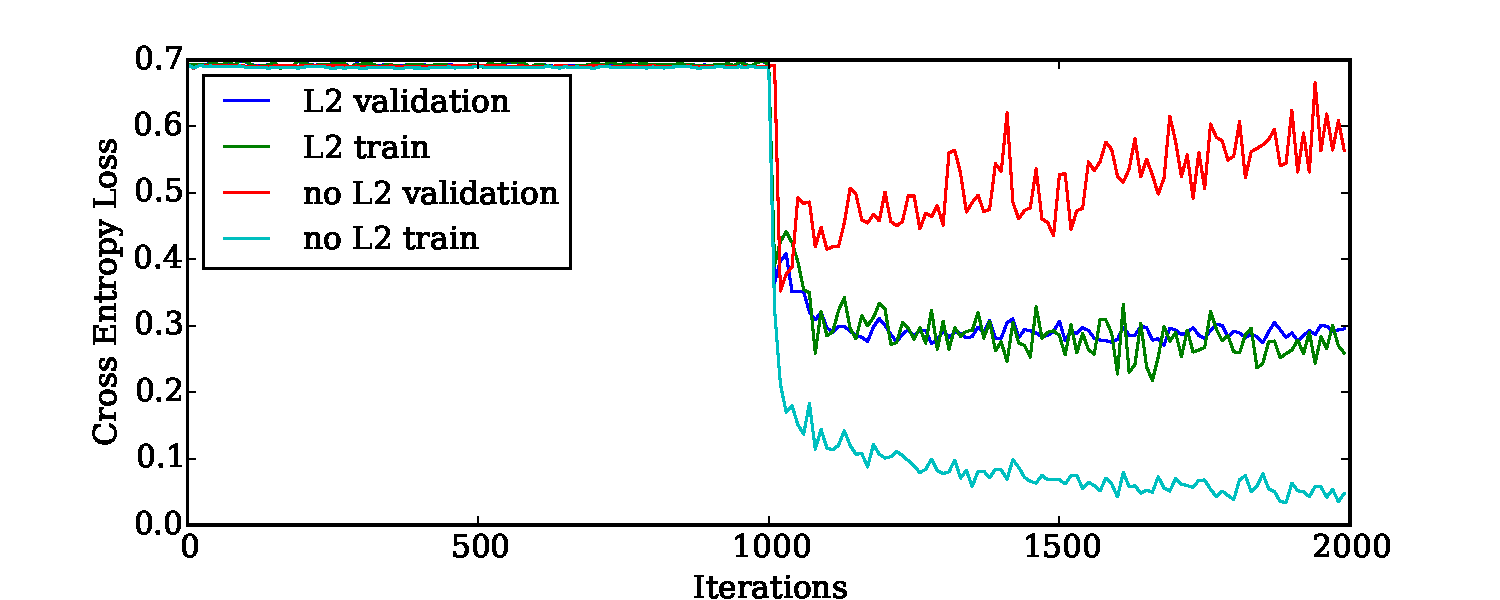
\includegraphics[width =0.8\hsize]{figures/l2.pdf}
    \caption{Plot of the classifier cross entropy loss losses of the two experiments in table \ref{tab:l2_2} }
    \label{fig:l2_1}
    \end{figure}

    \begin{figure}[!h]
    \centering
    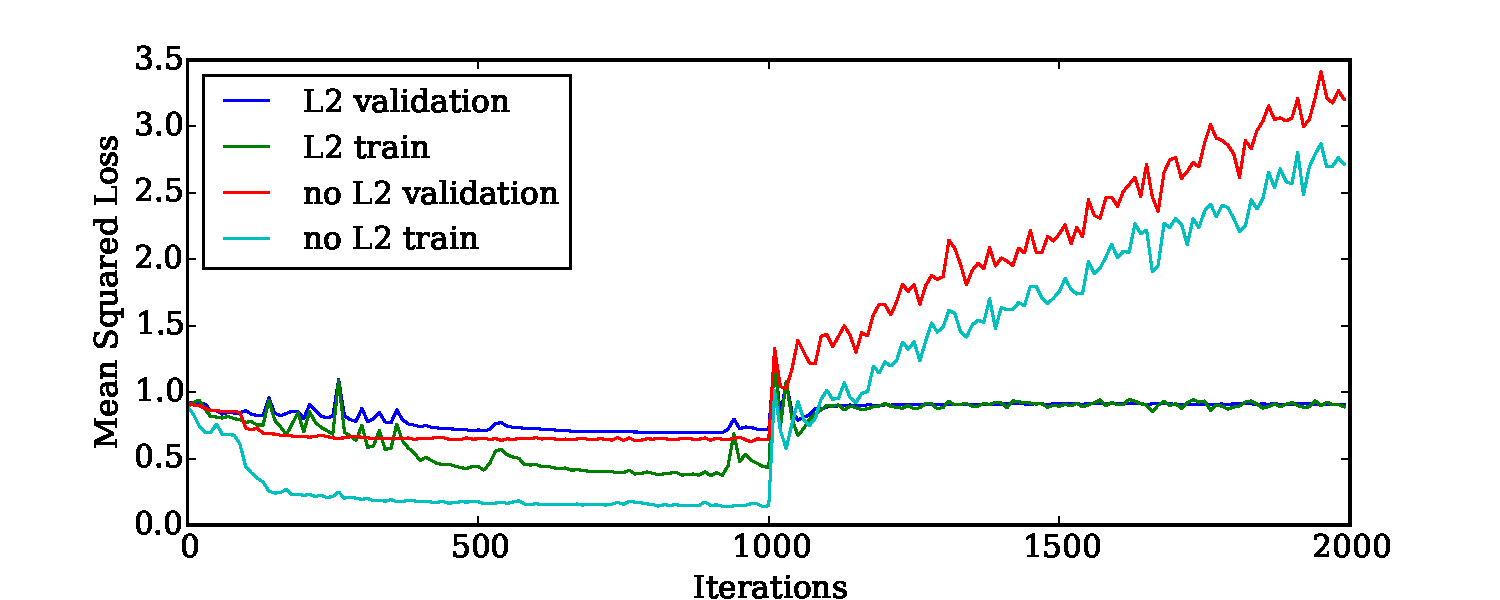
\includegraphics[width =0.8\hsize]{figures/l2_auto.pdf}
    \caption{Plot of the autoencoder mean squared loss of the two experiments in table \ref{tab:l2_2} }
    \label{fig:l2_2}
    \end{figure}

    With these results then, the conclusion is that including a small degree of L2
    Regularisation should be useful for exploring the aims of this project.


    %
    %
    %
    %
    %
    %
    \section{Autoencoder transfer functions}
    This section investgiates the autoencoder transfer functions described in section \ref{sec:autoalpha}.
    The classifier only situations are included as a baseline from which to compare
    what the autoencoder actually changes. The experimental question being asked here
    is whether the inclusion of the autoencoder can improve classification performance.



    \begin{table}[]
      \footnotesize{
      \centering
      \begin{tabular}{rrrrrrrrrrr}
                           &                      &                                                                              &                                                                              & \multicolumn{1}{r|}{}                                                       & \multicolumn{3}{c|}{Early Model}                                   & \multicolumn{3}{c|}{Final Model}                                   \\ \hline
      i                    & Network              & \multirow{2}{*}{\begin{tabular}[c]{@{}r@{}}Transfer \\ Function\end{tabular}} & \multirow{2}{*}{\begin{tabular}[c]{@{}r@{}}Total \\ Iterations\end{tabular}} & \multirow{2}{*}{\begin{tabular}[c]{@{}r@{}}Early \\ Iteration\end{tabular}} & ROC                  & F1                   & AE Loss              & ROC                  & F1                   & AE Loss              \\
      \multicolumn{1}{l}{} & \multicolumn{1}{l}{} &                                                                              &                                                                              &                                                                             & \multicolumn{1}{l}{} & \multicolumn{1}{l}{} & \multicolumn{1}{l}{} & \multicolumn{1}{l}{} & \multicolumn{1}{l}{} & \multicolumn{1}{l}{} \\ \hline
      2.1                 & 2                    &  step                 & 1500           & 1000    & 0.59  & 0.19 & 0.03  & 0.82 & 0.47 & 0.08  \\
      2.2                  & 2                    & alternate            & 1500           & 1000    & 0.81  & 0.46 & 0.1   & 0.82 & 0.47 & 0.12  \\
      2.3                  & 2                    & constant 0.5         & 1500           & 750     & 0.81  & 0.48 & 0.03  & 0.8  & 0.46 & 0.03  \\
      2.4                  & 2                    & sigmoid              & 1500           & 1000    & 0.8   & 0.46 & 0.03  & 0.79 & 0.46 & 0.03  \\
      2.5                  & 2                    & constant 0.0         & 1500           & 1000    & 0.8   & 0.47 & 0.56  & 0.79 & 0.46 & 0.64  \\
      2.6                  & 2                    & polynomial           & 1500           & 750     & 0.79  & 0.46 & 0.03  & 0.77 & 0.44 & 0.03  \\
      \hline
      3.1                  & 3                    & step                 & 1500           & 1000    & 0.38  & 0.19 & 0.03  & 0.81 & 0.45 & 0.18  \\
      3.2                  & 3                    & constant 0.5         & 1500           & 750     & 0.81  & 0.46 & 0.03  & 0.81 & 0.46 & 0.03  \\
      3.3                  & 3                    & sigmoid              & 1500           & 1000    & 0.8   & 0.46 & 0.03  & 0.8  & 0.44 & 0.04  \\
      3.4                  & 3                    & polynomial           & 1500           & 750     & 0.78  & 0.45 & 0.02  & 0.79 & 0.44 & 0.03  \\
      3.5                  & 3                    & constant 0.0         & 1500           & 1000    & 0.81  & 0.43 & 2.38  & 0.79 & 0.42 & 2.61  \\
      3.6                  & 3                    & alternate            & 1500           & 1000    & 0.69  & 0.32 & 0.1   & 0.77 & 0.37 & 0.23  \\
      \hline
      4.1                  & 4                    & constant 0.0         & 1500           & 1000    & 0.78  & 0.38 & 16.31 & 0.78 & 0.39 & 14.5  \\
      4.2                  & 4                    & step                 & 1500           & 1000    & 0.42  & 0.19 & 0.03  & 0.77 & 0.4  & 0.7   \\
      4.3                  & 4                    & constant 0.5         & 1500           & 750     & 0.73  & 0.33 & 0.03  & 0.75 & 0.36 & 0.03  \\
      4.4                  & 4                    & sigmoid              & 1500           & 1000    & 0.74  & 0.36 & 0.03  & 0.74 & 0.36 & 0.03  \\
      4.5                  & 4                    & polynomial           & 1500           & 750     & 0.52  & 0.21 & 0.09  & 0.67 & 0.3  & 0.04  \\
      4.6                  & 4                    & alternate            & 1500           & 1000    & 0.6   & 0.26 & 0.06  & 0.61 & 0.27 & 0.07  \\
      \hline
      \end{tabular}
      }
      \caption{Sorted by ROC perfomrance and secondarily by autoencoder loss.
      A comparison of the the autoencoder transfer functions with 0.8 dropout and local contrast normalisation layers (one for network 2 and two for networks 3 \& 4).
      Constant 0.5 means each cost function is trained equally, while constant 0.0 means training only of the classifier.
      Early model is just the evaulation at the early iteration and the final model is the evaluation of the network at the total number of iterations.
      The step function has its step at iteration 1000.
      The sigmoid function is $\alpha_{\text{sigmoid},1500,2/3,20}$
      The polynomial function is $\alpha_{\text{poly},1500,6}$.
      The alternate function is $\alpha_{\text{alternate}}(t,15000,2/3)$
      {\bf Experimental Configuration:} see caption for table \ref{tab:sharedweights}.} \label{tab:auto_final_1}
    \end{table}

      The first thing to note from the results in table \ref{tab:auto_final_1} is that
      the constant 0.0 experiments leave the autoencoder in a particularly dysfunctional state (with losses between 0.64 to 14.5),
      getting worse with the size of the network. Then there is the observation that
      the ROC scores are fairly close, with the F1 scores being almost the same. These two
      observations show that the two networks are achieving a very similar performance but
      with very different configurations. One explanation may be that the binary softmax layer weights
      contain a lot of information about classifying the AU's, if so then this suggests an
      instructive experiment for future work would be to only train these softmax weights to see
      what their maximum performance is. If they can achieve similar results then it may be possible
      the underlying convolution and max pooling layers are not fully helping to model the data.

      There is no obvious evidence that the smoother alpha functions contribute different
      dynamics. In these experiments, one possible issue is that
      the total amount of classifier and autoencoder training is not constant
      \footnote{In other words the area under the $\alpha(t)$ and $1-\alpha(t)$ curves are not constant between runs.}
      between transfer functions
      and this is something that might be critical for a really precise exposition. However the question of whether
      including the autoencoder is beneficial is still answerable.

      % [('polynomial', 6), ('alternate', 7), ('sigmoid', 10), ('constant 0.0', 10), ('constant 0.5', 13), ('step', 17)]
      Ranking the functions by their position in table \ref{tab:auto_final_1} scoring 6 for top place and 1 for worst place gives in order:
      step(17), constant 0.5 (13), constant 0.0 (10), sigmoid (10) and lastly alternate (7). Initially this indicates that the
      experiments including the autoencoder perform better but looking at the early models of the constant 0.0 experiments
      they often have very similar performance scores. So no substantial improvement is found.

      The losses for network 2 are plotted in appendix \ref{appendix2}.
